% (c) 2002 Matthew Boedicker <mboedick@mboedick.org> (original author) http://mboedick.org
% (c) 2003-2007 David J. Grant <davidgrant-at-gmail.com> http://www.davidgrant.ca
% (c) 2008 Nathaniel Johnston <nathaniel@nathanieljohnston.com> http://www.nathanieljohnston.com
% (l) 2012 Arun I B <arunib@smail.iitm.ac.in> http://www.ee.iitm.ac.in/~ee10s026/
%This work is licensed under the Creative Commons Attribution-Noncommercial-Share Alike 2.5 License. To view a copy of this license, visit http://creativecommons.org/licenses/by-nc-sa/2.5/ or send a letter to Creative Commons, 543 Howard Street, 5th Floor, San Francisco, California, 94105, USA.

\documentclass[letterpaper,11pt]{article}
\newlength{\outerbordwidth}
\pagestyle{empty}
\raggedbottom
\raggedright
\usepackage[svgnames]{xcolor}
\usepackage{framed}
\usepackage{times}
\usepackage{tocloft}
\usepackage{graphicx}
\usepackage{multirow}
\usepackage[utf8]{inputenc}
\usepackage{tabularx}
\usepackage{ctex}
\usepackage{verbatim}	%块注释
\usepackage{hyperref}%使用url

\title{Aparna-CV}
%-----------------------------------------------------------
%Edit these values as you see fit

\setlength{\outerbordwidth}{3pt}  % Width of border outside of title bars
\definecolor{shadecolor}{gray}{0.75}  % Outer background color of title bars (0 = black, 1 = white)
\definecolor{shadecolorB}{gray}{0.93}  % Inner background color of title bars


%-----------------------------------------------------------
%Margin setup

\setlength{\evensidemargin}{-0.25in}
\setlength{\headheight}{0in}
\setlength{\headsep}{0in}
\setlength{\oddsidemargin}{-0.25in}
\setlength{\paperheight}{11in}
\setlength{\paperwidth}{8.5in}
\setlength{\tabcolsep}{0in}
\setlength{\textheight}{9.5in}
\setlength{\textwidth}{7in}
\setlength{\topmargin}{-0.3in}
\setlength{\topskip}{0in}
\setlength{\voffset}{0.1in}


%-----------------------------------------------------------
%Custom commands
\newcommand{\resitem}[1]{\item #1 \vspace{-2pt}}
\newcommand{\resheading}[1]{\vspace{8pt}%{\vspace{8pt}
  \parbox{\textwidth}{\setlength{\FrameSep}{\outerbordwidth}
    \begin{shaded}
\setlength{\fboxsep}{0pt}\framebox[\textwidth][l]{\setlength{\fboxsep}{4pt}\fcolorbox{shadecolorB}{shadecolorB}{\textbf{\sffamily{\mbox{~}\makebox[6.762in][l]{\large #1} \vphantom{p\^{E}}}}}}
    \end{shaded}
  }\vspace{-5pt}%\vspace{-5pt}
}
\newcommand{\ressubheading}[4]{
\begin{tabular*}{6.5in}{l@{\cftdotfill{\cftsecdotsep}\extracolsep{\fill}}r}
		\textbf{#1} & #2 \\
		\textit{#3} & \textit{#4} \\
\end{tabular*}\vspace{-6pt}}
%-----------------------------------------------------------

\begin{document}

%-----------------------------------------------------------
%Insert IIT Madras Logo 
\begin{tabular*}{7in}{l@{\extracolsep{\fill}}r}
  & \multirow{4}{*}{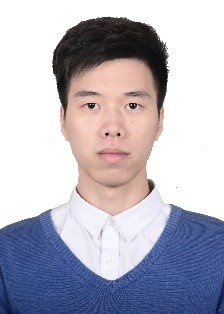
\includegraphics[scale=0.95]{hjh.jpg}}\\%  & \multirow{4}{*}{\includegraphics[scale=0.19]{iitmlogo}}
  & \\
%-----------------------------------------------------------  
  \textbf{\Large Junhao Huang} & \\% $|$ EE10S0600 
%   PhD Student& \\%Research Scholar
%   Beijing Normal University-Hong Kong Baptist University United International College (UIC)  \\
  Phone: +86-18626423381, Email: jhhuang\_nuaa@126.com \\
  Homepage: https://junhaohuang.github.io/
\end{tabular*}
\\


%%%%%%%%%%%%%%%%%%%%%%%%%%%%%%
\resheading{Education}
%%%%%%%%%%%%%%%%%%%%%%%%%%%%%%

\begin{itemize}
\item
	\ressubheading{BNU-HKBU United International College}{Supervisor: Dr. Donglong Chen}{PhD Degree of Hong Kong Baptist University}{Sep. 2021-now}
\begin{comment}%开始注释
	\begin{itemize}
		\resitem{Major Courses: Mathematical foundation of information security, Modern Cryptography and Application, Blockchain Application, Digital Design and Computer architecture.}
	\end{itemize}
\end{comment}%结束注释
\item
	\ressubheading{Nanjing University of Aeronautics and Astronautics}{Supervisor: Prof. Zhe Liu}{Master Degree of Cyberspace Security}{Sep. 2018-Jun. 2021}
\begin{comment}%开始注释
	\begin{itemize}
		\resitem{Major Courses: Mathematical foundation of information security, Modern Cryptography and Application, Blockchain Application, Digital Design and Computer architecture.}
	\end{itemize}
\end{comment}%结束注释

\item
	\ressubheading{Nanjing University of Aeronautics and Astronautics}{GPA: 3.7}{Bachelor Degree of Computer Science and Technology}{Sep. 2014-Jun. 2018}
\begin{comment}%开始注释
	\begin{itemize}
		\resitem{Major Courses: C/C++, Data Structure, Algorithm Design, Software Engineering, Computer Organization and Assembly Language, Operating System.}
	\end{itemize}
\end{comment}%结束注释

\end{itemize}

\begin{comment}%开始注释
\begin{itemize}
\item
	\ressubheading{My University}{My Town,}{B.Sc. Physics}{2004 - 2008}
	\begin{itemize}
		\resitem{Undergraduate Thesis: Why Electron Spins Rule}
		\resitem{Graduated with Honours and a XX.X\% average}
	\end{itemize}

\item
	\ressubheading{My High School}{Hick Town, ON}{High School Diploma}{2000 - 2004}
	\begin{itemize}
		\resitem{President of Students' Council and captain of the rugby team in senior year}
		\resitem{Graduated with a XX.X\% average}
	\end{itemize}
\end{itemize}
\end{comment}%结束注释
%%%%%%%%%%%%%%%%%%%%%%%%%%%%%%
\resheading{Research Interest}
%%%%%%%%%%%%%%%%%%%%%%%%%%%%%%
\begin{itemize}
\item
	Cryptographic Engineering, Post-quantum Cryptography, Lattice-based Cryptography, Modular Arithmetic.

\end{itemize}


%%%%%%%%%%%%%%%%%%%%%%%%%%%%%%
\resheading{Representative Publications (Total: 13)}
%%%%%%%%%%%%%%%%%%%%%%%%%%%%%%
\begin{enumerate}\setlength{\itemsep}{0pt}
	\item {Yet another Improvement of Plantard Arithmetic for Faster Kyber on Low-end 32-bit IoT Devices,\\
	\textbf{Junhao Huang}, Haosong Zhao, Jipeng Zhang, Wangchen Dai, Lu Zhou, \c{C}etin Kaya Ko\c{c}, Ray C.C. Cheung, Donglong Chen*. \\
	In \textcolor{blue}{IEEE Transactions on Information Forensics \& Security, 2024.} (\textbf{CCF-A, 安全顶刊})
	}
	\item {Revisiting Keccak and Dilithium Implementations on ARMv7-M,\\
	\textbf{Junhao Huang}, Alexandre Adomnicăi, Jipeng Zhang, Wangchen Dai, Yao Liu, Ray C. C. Cheung, \c{C}etin Kaya Ko\c{c}, Donglong Chen*. \\
	In \textcolor{blue}{IACR Transactions on Cryptographic Hardware and Embedded Systems, 2024.} (\textbf{CCF-B, 密码顶会})
	}
	\item {Improved Plantard Arithmetic for Lattice-based Cryptography,\\
	\textbf{Junhao Huang}, Jipeng Zhang, Haosong Zhao, Zhe Liu, Ray C. C. Cheung, \c{C}etin Kaya Ko\c{c}, Donglong Chen*. \\
	In \textcolor{blue}{IACR Transactions on Cryptographic Hardware and Embedded Systems, 2022.} (\textbf{CCF-B, 密码顶会})
	}
	\item {ENG25519: Faster TLS 1.3 handshake using optimized X25519 and Ed25519,\\ 
	Jipeng Zhang, \textbf{Junhao Huang}, Lirui Zhao, Donglong Chen, Çetin Kaya Koç*.\\ 
	In \textcolor{blue}{Usenix Security, 2024.} (\textbf{CCF-A, 安全四大顶会, Distinguished Paper Award})
	}
	\item {Optimized Software Implementation of Keccak, Kyber, and Dilithium on RV\{32,64\}IM\{B\}\{V\},\\
		Jipeng Zhang, Yuxing Yan, \textbf{Junhao Huang}, Çetin Kaya Koç*.\\ 
		In \textcolor{blue}{IACR Transactions on Cryptographic Hardware and Embedded Systems, 2025.} (\textbf{CCF-B, 密码顶会})
	}
	\item {ECO-CRYSTALS: Efficient Cryptography CRYSTALS on Standard RISC-V ISA.\\
	Xinyi Ji, Jiankuo Dong, \textbf{Junhao Huang}, Zhijian Yuan, Wangchen Dai, Fu Xiao, Jingqiang Lin.\\  In \textcolor{blue}{IEEE Transactions on Computers, 2024.} (\textbf{CCF-A})
	}
	\item {Time-memory Trade-offs for Saber on Memory-constrained RISC-V,\\
	Jipeng Zhang, \textbf{Junhao Huang}, Zhe Liu*, Sujoy Sinha Roy. \\
	In \textcolor{blue}{IEEE Transactions on Computers, 2022.} (\textbf{CCF-A})
	}
	\item {Parallel Implementation of SM2 Elliptic Curve on Intel Processor with AVX2. \\\textbf{Junhao Huang}, Zhe Liu*, Zhi Hu, and Johann Großschädl. \\ In \textcolor{blue}{Australasian Conference on Information Security and Privacy - ACISP 2020.} (\textbf{CCF-C})
	}

\end{enumerate}

% %%%%%%%%%%%%%%%%%%%%%%%%%%%%%%
% \resheading{Reaserch Experiences}
% %%%%%%%%%%%%%%%%%%%%%%%%%%%%%%
% \begin{itemize}
% 	\item
% 	Jul. 2023- Oct. 2023,\quad Revisiting Keccak and Dilithium Implementations on ARMv7-M
% % \begin{comment}%开始注释
% 	\begin{itemize}
% 		\resitem{Further improve Keccak's performance using lazy rotation and better memory access scheduling on ARMv7-M.}
% 		\resitem{Efficient multi-moduli NTT with Plantard arithmetic for the small polynomial multiplication in Dilithium on ARM Cortex-M3.}
% 		\resitem{Obtain large speed-ups for Keccak and Dilithium on Cortex-M3 and Cortex-M4.}
% 	\end{itemize}
% 	\item
% 	Sep. 2022- Mar. 2023,\quad Yet another Improvement of Plantard Arithmetic for Faster Kyber on Low-end 32-bit IoT Devices
% % \begin{comment}%开始注释
% 	\begin{itemize}
% 		\resitem{Further extend the input range of the improved Plantard arithmetic tailored for Kyber.}
% 		\resitem{Efficient NTT/INTT implementation on Cortex-M3 and RISC-V.}
% 		\resitem{Speed-ups for Kyber on Cortex-M3 and RISC-V.}
% 	\end{itemize}
% 	\item
% 	Sep. 2021- Apr. 2022,\quad Improved Plantard Arithmetic for Lattice-based Cryptography
% % \begin{comment}%开始注释
% 	\begin{itemize}
% 		\resitem{Present an improved Plantard arithmetic tailored for LBC.}
% 		\resitem{Obtained speed-ups for Kyber and NTTRU with 16-bit NTT on Cortex-M4.}
% 		\resitem{The source code has been merged into \href{https://github.com/mupq/pqm4/pull/244}{pqm4, PR\#244} (merged at 25th, Oct, 2022).}
% 	\end{itemize}

% 	\item
% 	Dec. 2020- Apr. 2021,\quad Memory Efficient Implementation of Saber on RISC-V
% % \begin{comment}%开始注释
% 	\begin{itemize}
% 		\resitem{Reduce the memory usage of Saber by using a \textbf{just-in-time} public matrix, secret, and noise generation technique.}
% 		\resitem{Represent the secret, and noise with a new \textbf{smaller data-type}, which reduces the size of the secret and noise.}
% 	\end{itemize}
	% \item
% 	Apr. 2019- Nov. 2020,\quad Accelerating ECC utilizing the Double Precision Floating-point Number on GPU
% % \begin{comment}%开始注释
% 	\begin{itemize}
% 		\resitem{Implement the prime field arithmetic for the prime modulus $p=2^n-\delta$ by combining the computing power of \textbf{the fused multiply-add instruction of double-precision floating-point number} and the addition, subtraction, and shift instructions of integer number. }
% 		\resitem{Propose how to perform multi-precision multiplication over unreduced-form big number, which optimizes the point multiplication, especially Montgomery ladder algorithm for Montgomery curves, with the \textbf{lazy reduction technique}.}
% 	\end{itemize}
% 	\item
% 	Sep. 2019- Mar. 2020,\quad Accelerating SM2 on GPU
% % \begin{comment}%开始注释
% 	\begin{itemize}
% 		\resitem{Implement the prime field arithmetic for SM2 using the low-level PTX assembly language on GPU, which contributes to the performance of the high-level point arithmetic and cryptographic protocols of SM2.}
% 	\end{itemize}
% 	\item
% 	Apr. 2019- Oct. 2019,\quad Parallel Implementation of SM2 Elliptic Curve with AVX2
% % \begin{comment}%开始注释
% 	\begin{itemize}
% 		\resitem{Utilize SIMD AVX2 instruction set to implement 2-way SM2 prime field operations.}

% 		\resitem{Reschedule the (X,Y)-only Co-Z Jacobian arithmetic and perform the symmetric operations using the 2-way prime field operations}

% 		\resitem{Implement the Co-Z based Montgomery ladder algorithm based on the parallel Co-Z Jacobian arithmetic.}

% 		\resitem{The number of the 2-way prime field operations of the Co-Z Jacobian arithmetic is reduced to a half compared to the sequential implementation.}

% 		\resitem{The AVX2 version Co-Z based Montgomery ladder algorithm is \textbf{1.31} times faster than the X64 assembly implementation.}
% 	\end{itemize}
% \item 
% 	Nov. 2016- Mar. 2017\quad University Association Information Management System (APP)
% 	\begin{itemize}
% 		\resitem{An app that facilitates internal communication and management of associations, and simplifies members' participation in association activities.}
% 		\resitem{Achieve Association management, Association activities management, Association member management.}
% 		\resitem{Applied for a \textbf{Software Copyright}.}
% 	\end{itemize}
% \end{itemize}

%%%%%%%%%%%%%%%%%%%%%%%%%%%%%%
\resheading{Research Activities}
%%%%%%%%%%%%%%%%%%%%%%%%%%%%%%
\begin{itemize}
\item
	\ressubheading{IACR CHES/TCHES 2024 Artifact Evaluation Committee}{Halifax, Canada}{ International Association for Cryptologic Research (IACR)}{Oct. 2023-Oct. 2024}
\item
	\ressubheading{Visiting Scholar, Electrical Engineering}{Hong Kong, China}{City University of Hong Kong, Prof. Ray C. C. Cheung}{Jul. 2023-Dec. 2023}
% \item
% 	\ressubheading{Teaching Assistant}{Zhuhai, China}{BNU-HKBU UIC, Operating Systems, Dr. Sunny Seon Phil JEONG}{Feb. 2023-Jun. 2023}
% \item
% 	\ressubheading{Teaching Assistant}{Zhuhai, China}{BNU-HKBU UIC, Computer and Network Security, Dr. Donglong Chen}{Sep. 2021-Dec. 2021}
\item
	\ressubheading{Visiting Scholar, Cyberspace Security}{Whuhan, China}{Wuhan University, Prof. Debiao He}{Sep. 2019-Jan. 2020}

\end{itemize}

%%%%%%%%%%%%%%%%%%%%%%%%%%%%%%
\resheading{Honor Certificates}
%%%%%%%%%%%%%%%%%%%%%%%%%%%%%%
\begin{itemize}
\item 
	Aug. 2024\quad   \textbf{Distinguished Paper Award} of the 33rd USENIX Security Symposium.
\item 
	May. 2023\quad   Third prize for the Guangdong Province Cyberspace Security Outstanding Paper Award, GDCA.
\item 
	Apr. 2023\quad   Best RPG Poster Award of Faculty of Science \& Technology, BNU-HKBU UIC.
% \item 
	% Nov. 2019\quad   Patent for An efficient implementation of Co-Z based Montgomery ladder algorithm using AVX2, CN112367172A.
% \item
% 	Oct. 2018\quad	Postgraduate \textbf{First prize} Scholarship
% \item
% 	Oct. 2018\quad	\textbf{First Prize} of Academic Scholarship
% \item
	% Jun. 2018\quad	Software Copyright for the University Association Information Management System
% \item
% 	Oct. 2017\quad	National Encouragement Scholarship, \textbf{Third Prize} of Outstanding Student Scholarship
% \item
% 	Oct. 2016\quad	National Encouragement Scholarship, \textbf{Second Prize} of Outstanding Student Scholarship
% \item
	% Oct. 2015\quad	National Encouragement Scholarship, \textbf{First Prize} of Outstanding Student Scholarship
\end{itemize}


%%%%%%%%%%%%%%%%%%%%%%%%%%%%%%
\resheading{Professional Skills}
%%%%%%%%%%%%%%%%%%%%%%%%%%%%%%
\begin{enumerate}\setlength{\itemsep}{0pt}
	\item {Language Level: CET-4: 597, CET-6: 513, IELTS: 7.0}
	\item {Skills: C/C++, x86-64, ARM, RISC-V, AVX2, CUDA, Python}
\end{enumerate}

% % \begin{comment}%开始注释
% %%%%%%%%%%%%%%%%%%%%%%%%%%%%%%
% \resheading{Self Introduction}
% %%%%%%%%%%%%%%%%%%%%%%%%%%%%%%
%   \begin{center}
%   \parbox{6.762in}{I have been implementing elliptic curve cryptography since I was a graduate student. I tried to implement SM2 and other elliptic curves using different languages on different platforms, i.e. C, x86-64 assembly language, AVX2 on CPU, and CUDA programming on GPU. During the 5-month exchange study at Wuhan University, Lattice-based Cryptography and Blockchain are two other research areas of my interest. Recently, I've been trying to implement Kyber on a RISC-V chip, which further expands my experiences on cryptographic engineering.}
%   \end{center}
% \end{comment}%结束注释
\end{document}